\documentclass[tikz,border=10pt]{standalone}
\usetikzlibrary{shapes,arrows.meta,positioning}

\begin{document}
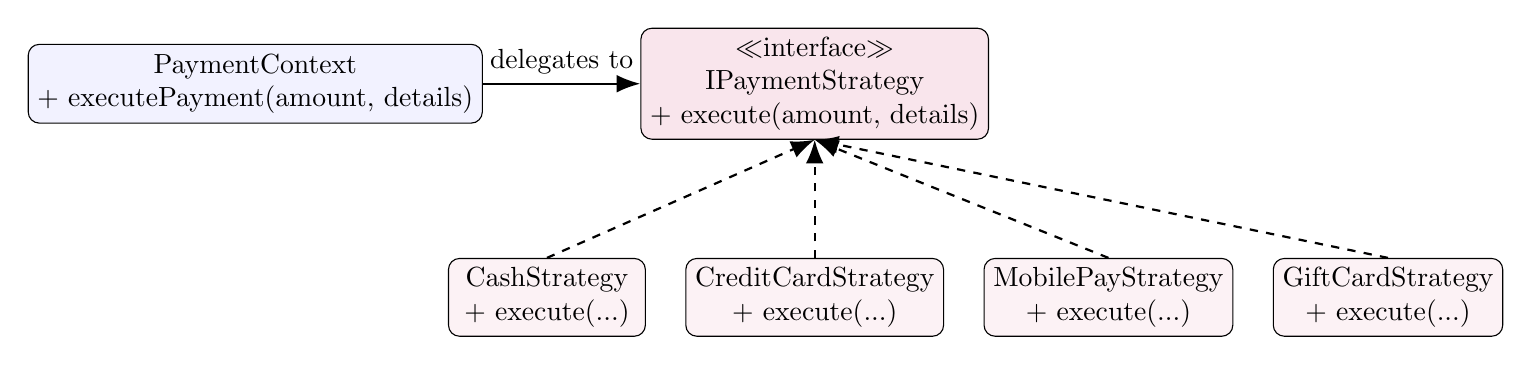
\begin{tikzpicture}[
    box/.style={draw, rectangle, rounded corners, minimum width=3cm, minimum height=1cm, align=center, fill=blue!5},
    strategy/.style={draw, rectangle, rounded corners, minimum width=3cm, minimum height=1cm, align=center, fill=purple!10},
    concrete/.style={draw, rectangle, rounded corners, minimum width=2.5cm, minimum height=0.8cm, align=center, fill=purple!5},
    arrow/.style={-{Latex[length=3mm]}, thick},
    dashedarrow/.style={-{Latex[length=3mm]}, dashed, thick}
]

\node[box] (context) {PaymentContext\\+ executePayment(amount, details)};
\node[strategy, right=2cm of context] (interface) {$\ll$interface$\gg$\\IPaymentStrategy\\+ execute(amount, details)};

\node[concrete, below=1.5cm of interface] (credit) {CreditCardStrategy\\+ execute(...)};
\node[concrete, left=0.5cm of credit] (cash) {CashStrategy\\+ execute(...)};
\node[concrete, right=0.5cm of credit] (mobile) {MobilePayStrategy\\+ execute(...)};
\node[concrete, right=0.5cm of mobile] (gift) {GiftCardStrategy\\+ execute(...)};

\draw[arrow] (context) -- node[above] {delegates to} (interface);
\draw[dashedarrow] (cash.north) -- (interface.south);
\draw[dashedarrow] (credit.north) -- (interface.south);
\draw[dashedarrow] (mobile.north) -- (interface.south);
\draw[dashedarrow] (gift.north) -- (interface.south);

\end{tikzpicture}
\end{document}
